\documentclass[9pt]{beamer}


\usepackage{introLatex}
\usepackage{shortcutLatex}
\usepackage{layout}
\usepackage{algorithm}
\usepackage{algorithmic}


% Dossier où se trouvent les images
\graphicspath{{imagesdiapo/}}


\newcommand{\widesim}[2][1.5]{
  \mathrel{\underset{#2}{\scalebox{#1}[1]{$\sim$}}}
  }


\begin{document}

	\begin{frame}[t]
	\titlepage
	\end{frame}


	\begin{frame}
	\vspace*{22pt}
	\tableofcontents
	\end{frame}





\footHeadLine{}

\section{Introduction du problème}

\subsection{Physique statistique et modèle d'Ising}

\setlength{\columnseprule}{0.4pt}
\begin{frame}
		\justifying
		\vspace*{22pt}


\begin{multicols}{2}

		$\bullet$ Modèle d'Ising 2D carré :
			$N_s$ spins à une composante sur un quadrillage
			\vspace*{-11pt}
			
\begin{figure}[H]
\begin{center}
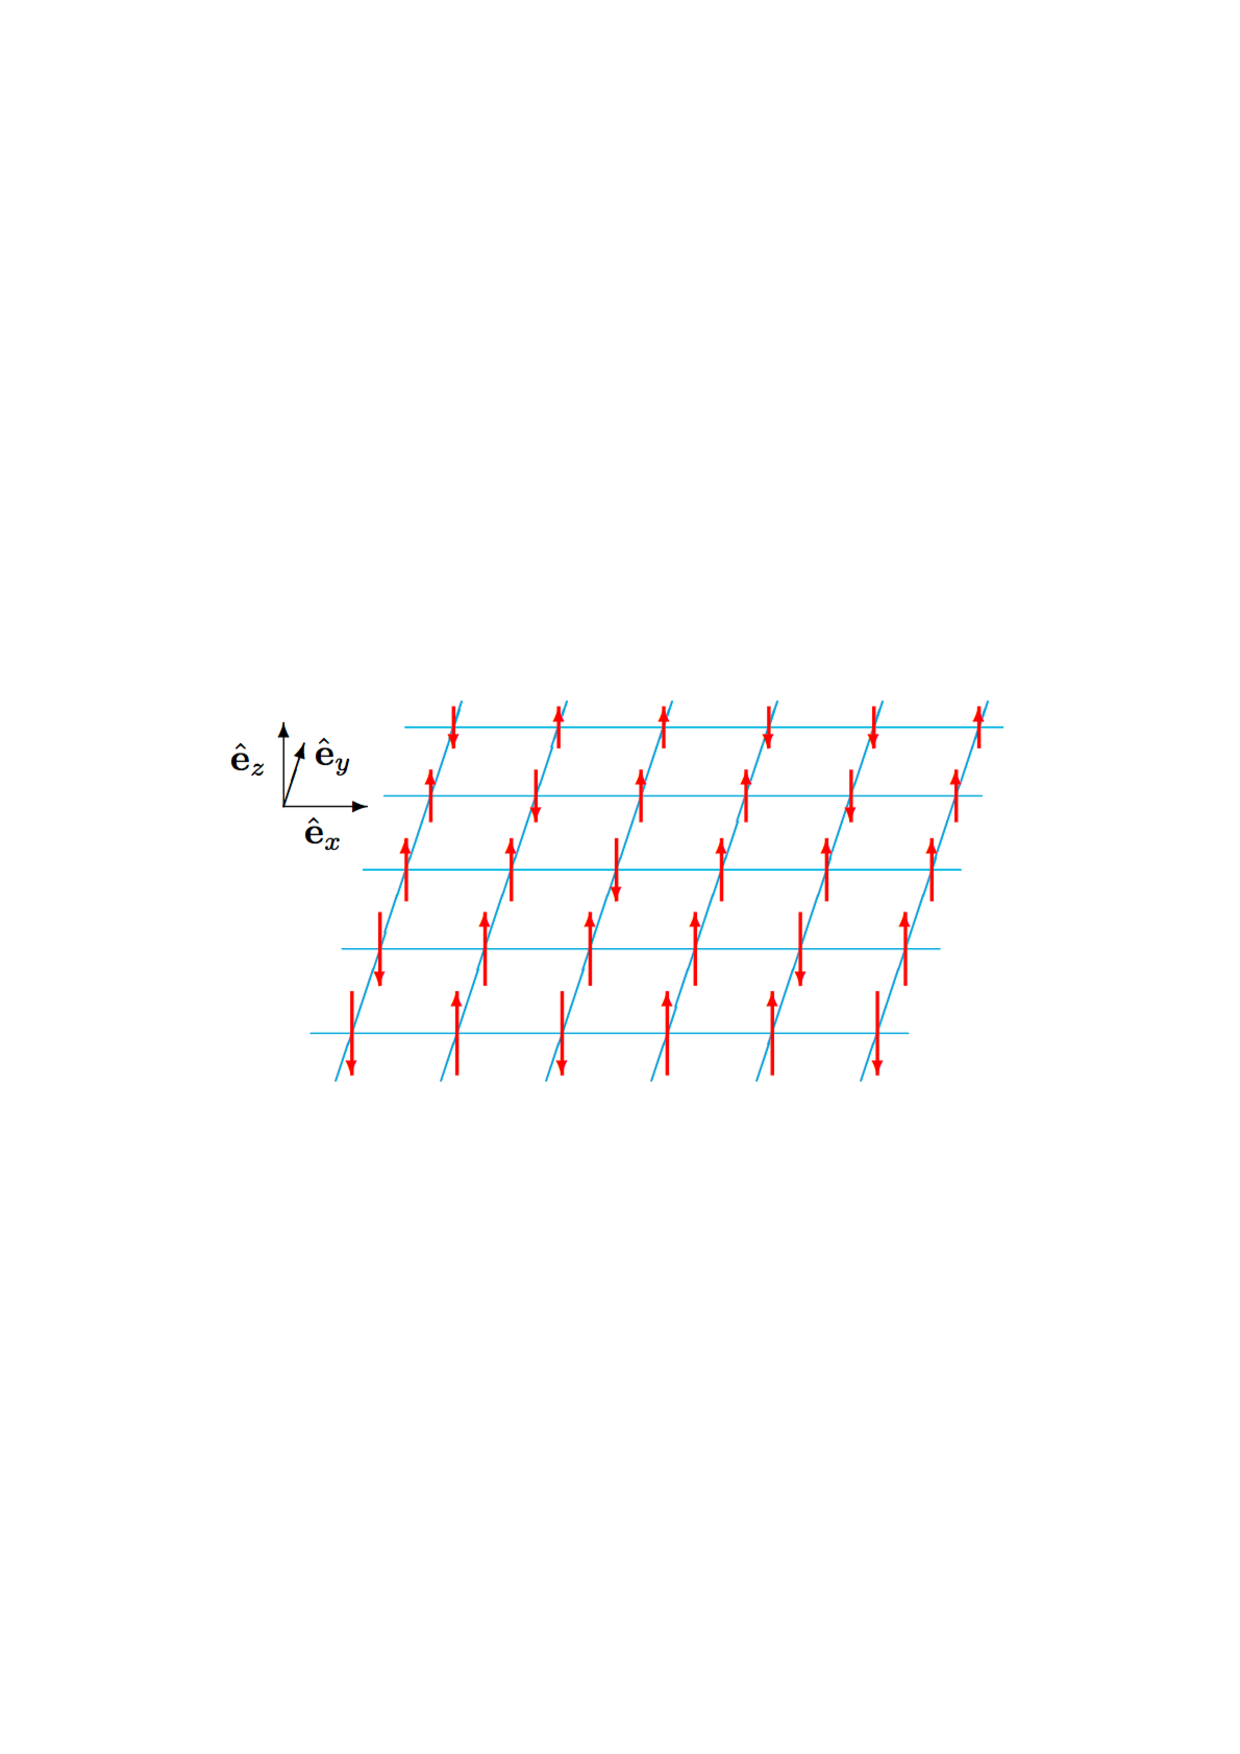
\includegraphics[scale =0.35]{Ising2D.pdf}
\caption{Modèle d'Ising.}
	\label{fig:schemaIsing}
	\end{center}
\end{figure}

$\bullet$ Spin et configuration :
\begin{equation*}
 S_\rv \in \{-1(\downarrow),1(\uparrow)\}, \quad \Mr = \{S_\rv\}_\rv
\end{equation*}


$\bullet$ Energie d'une config. $\Mr$ : $ \Hc(\Mr,b)$ \\
\commentout{\begin{equation*}
  \Hc(\Mr) = \sum_{\left< \rv, \rv' \right>} S_\rv S_{\rv'} - \sum_\rv b_\rv S_\rv	
\end{equation*}}

\vspace*{11pt}
$\bullet$ Probabilité d'une config. $\Mr$ :
\begin{equation*}
p(\Mr,b, T) = \frac{1}{\Zc} \exp\(-\frac{\Hc(\Mr,b)}{k_BT}\)
\end{equation*}
$\bullet$ Fonction de partition :
\begin{equation*}
\Zc(b,T) = \sum_\Mr \exp\(-\frac{\Hc(\Mr,b)}{k_BT}\)
\end{equation*}
\vfill

	\end{multicols}
\end{frame}

\begin{frame}
		\justifying
		\vspace*{22pt}
	$\bullet$	Définition de l'aimantation :  
		\begin{equation*}
			m = \sum_{\Mr = \{S_\rv\}_\rv }  \left\{p(\Mr,b) \( \frac{1}{N_s} \sum_\rv S_\rv\) \right\}  = \frac{1}{N_s\beta}\partial_\beta \ln\(\Zc \) 
		\end{equation*}
		
	\onslide<2->{	
		\vspace*{11pt}
		$\bullet$ Evolution de l'aimantation $m$ avec la température $T$ :
		
\begin{multicols}{2}


	\begin{figure}[H]
\begin{center}
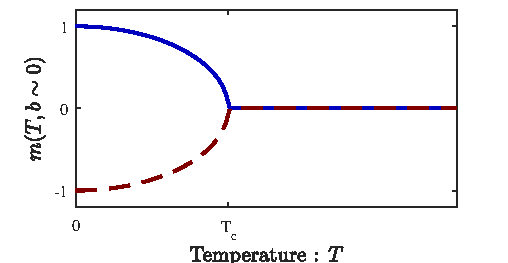
\includegraphics[width =0.95\columnwidth]{aimantation.pdf}
\caption{Aimantation $m$ vs $T$}
	\label{fig:schemaIsing}
	\end{center}
\end{figure}
	
	\vspace*{-11pt}
	Invariance par échange de $\ev_z$ en $-\ev_z$ :\\
	$\Hc(\Mr,b=0) = \Hc(-\Mr,b=0)$ \\
	$\quad \diamond$ symétrie $\mathbb{Z}_2$ \\
	$\quad \diamond$ à $(b = 0, T=0)$  : $m=0$. \\
	\vspace*{8pt}}
	\onslide<3->{
	Mais problème : 
	\begin{equation*}
		\lim_{N_s \to \infty} \(\lim_{b \to 0} m \) = 0 \neq \lim_{b \to 0} \( \lim_{N_s \to \infty} m \)
	\end{equation*}
	
	\end{multicols}
	}
	\onslide<4->{
	\begin{center}
$\Rightarrow$ {\Large Brisure de symétrie \& Transition de phase }
\end{center}
		}
\end{frame}
    



\subsection{Transition de phase}

	\begin{frame}
		\justifying
		\vspace*{22pt}


\onslide<1->{$\bullet$ Température critique : $T_c$} \\
\vspace*{11pt}
\onslide<2->{$\bullet$ Transitions de phase du second ordre : \\


$\quad \diamond$ Fonction de corrélation à deux points :
\begin{equation*}
\begin{split}
	G^{(2)}(|\rv_1 - \rv_2|) & \equiv \left< S_{\rv_1} S_{\rv_2} \right>   \equiv \sum_{\Mr}  p\(\Mr\) S_{\rv_1} S_{\rv_2} \, 
	\end{split}
\end{equation*}
$\quad \diamond$ Longueur de corrélation $\xi$ : 
\begin{equation*}
G^{(2)}(r >\xi) \simeq 0 \quad \text{et} \quad G^{(2)}(r < \xi) \neq 0
\end{equation*}
\vspace*{2pt}
}

\onslide<3->{
$\bullet$ Exposants critiques $\eta$ et $\nu$ :
\begin{equation*}
	\xi \widesim{T \to T_c} |T-T_c|^{-\nu} \quad \text{et à } T = T_c, \quad	 G^{(2)}(r) \widesim{r \to \infty} |r|^{2-d-\eta}
\end{equation*}

}

\onslide<4->{
\begin{center}
$\Rightarrow$ {\Large Universalité des exposants critiques }
\end{center}
}

	\end{frame}


\setlength{\columnseprule}{0pt}


\commentout{
	\begin{frame}
		\justifying
		\vspace*{22pt}

$\bullet$ Fonction de partition exprimée avec des champs :
\begin{equation*}
	\Zc = \int \Dc \varphiv \exp\(-\Hc[\varphiv]/(k_BT)\)
\end{equation*}


\begin{multicols}{2}

$\bullet$ Transformée de Fourier :
\vspace*{-11pt}
\begin{equation*}
\begin{split}
\hat{\varphiv}_\pv = \frac{1}{\sqrt{|\Omega|}}\int_\Omega \varphiv(\rv) \, e^{-i \pv . \rv} \dd \, \rv, \\
\varphiv(\rv) = \frac{1}{\sqrt{|\Omega|}}\sum_\pv \hat{\varphiv}_\pv \, e^{i \pv  .\rv}
\end{split} 	
\end{equation*}
$ \bullet $ $\|\pv \|_2 \in [0, \Lambda]$
\vspace*{22pt}
\begin{figure}
\begin{center}
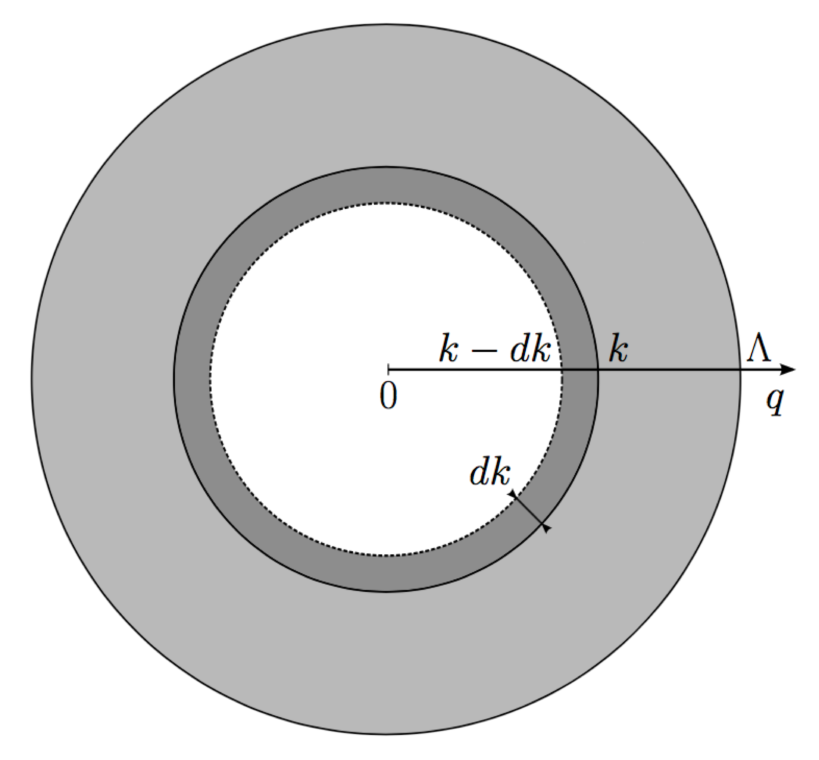
\includegraphics[scale = 0.3]{SchemaRG.pdf}
\caption{Principe du RG \\ {\footnotesize \textit{Thèse de Frédéric Léonard}}}
	\label{fig:SchemaRG}
	\end{center}
\end{figure}

\end{multicols}

	$\bullet$ En pratique :  $\Zc_k \underset{\text{NPRG}}{\longrightarrow} \Gamma_k   \underset{\text{BMW}}{\longrightarrow} \Gamma^{(2)}_k$
	\end{frame}
	
}

    
    \subsection{Objectifs}
    \begin{frame}
		\justifying
		\vspace*{22pt}
    
    \onslide<1->{$\Rightarrow$ {\Large Calcul des exposants critiques : $\eta$ et $\nu$ } }\\
    \onslide<2->{$\Rightarrow$ {\Large Calcul de la température critique : $T_c$ }} \\
    
    \vspace*{11pt}
    
    \onslide<3->{
    $\bullet$ Première étude :\\
    \begin{itemize}
    \item Réecriture en C++ d'un code permettant de calculer $\eta$ et $\nu$
    \item Recherche des problèmes et tentatives de résolution
    \end{itemize}
    }
    
    \vspace*{11pt}
    
    \onslide<4->{
    $\bullet$ Deuxième étude :\\
    \begin{itemize}
    \item Ecriture d'un nouveau code pour calculer $T_c$ : faisable  mais difficile
    \item Comparaison à la valeur théorique : benchmarking de la méthode
    \end{itemize}
    }
    
    \end{frame}

    
 \commentout{   

    
    \section{Le problème continu}
    \subsection{Hamiltonien du modèle continu $\varphiv^4$}
    
        \sommaire{}
    
    
      \begin{frame}
		\justifying
		\vspace*{22pt}
    
    \begin{equation}
		H[\varphiv] = \int_\rv \, \left\{ \frac{1}{2}(\nabla \varphiv)^2 + \frac{1}{2}r_0 \varphiv^2 + \frac{u_0}{4!}{\({\varphiv}^{2}\)}^{2} \right\}
		\label{eq:hamiltCont}
\end{equation}
    	\end{frame}
    
    
    \subsection{Système d'équations à résoudre}
    
    
    \begin{frame}
		\justifying
		\vspace*{22pt}

{\itshape Trouver $(\tY_k,\tW_k)$ tel que pour tout $k \in ]0 ,\Lambda]$,  $\trho \in [0, +\infty[$ et $\tp \in [0, +\infty[$,}
\begin{align*}
	\partial_t  \tY_k(\tp, \trho) & = 
	\begin{aligned}[t]
			& \eta_k(1+\tY_k(\tp, \trho)) + \tp \, \partial_{\tp} \tY_k(\tp, \trho)  -(2-d-\eta_k)\trho \,\partial_{\trho} \tY_k(\tp, \trho)  \quad  \\
			& + 2\trho \tp^{-2} \left[ {\( \tp^2 \partial_{\trho} \tY_k(\tp, \trho) + \tilde{u}_k(\trho)\)}^2\, \tJ_3(\tp, \trho) \right]  - 2\trho \tp^{-2} \left[ \tilde{u}_k^2(\trho)  \tI_3(\trho) \right] \\
			&  - \tI_2(\trho) \(  \partial_{\trho} \tY_k(\tp, \trho) / 2 + \trho \,  \partial_{\trho}^2 \tY_k(\tp, \trho) \)
	\end{aligned}
	\label{eqn}\\
	\partial_t  \tW_k &  = 
	\begin{aligned}[t]
		& (\eta_k-2) \tW_k(\trho) + (d-2+\eta_k) \trho \,\partial_{\trho}\tW_k(\trho) + \frac{1}{2} \partial_{\trho} \tI_1(\trho) \, ,
	\end{aligned}
\end{align*}
\textit{avec la définition}
\begin{equation*}
\begin{split}
\eta_k = \frac{1}{2}  \tI_2(\trho = 0)\partial_\rho\tY_k(\tp = 0, \trho = 0) \,, 
\end{split}
\end{equation*}
\textit{et les conditions initiales,}
\begin{equation*}
	\tY_\Lambda(\tp, \trho) = 0 \quad  \text{et} \quad \tW_\Lambda(\trho) = \tilde{r}_0 + \tilde{u}_0\trho
\end{equation*}

	\end{frame}
	

	\subsection{Méthodes numériques}
	
	
     \begin{frame}
		\justifying
		\vspace*{22pt}
    
    
   	\onslide<1->{$\bullet$ Discrétisation en temps : Schéma d'Euler explicite} \\
   	\onslide<2->{$\bullet$ Discrétisation en champ : Grille fixe. Dérivée avec schémas à 5 points}\\
   	\onslide<3->{$\bullet$ Discrétisation en moments : Méthode pseudo-spectrale
   	\begin{itemize}
   		\item Interpolation de Tchebytechev	
   		\item Intégration de Gauss-Legendre
   	\end{itemize}
 } 	
   	\vspace*{11pt}
   
   \onslide<4->{	
   	$\bullet$ A propox de l'intégration
   	\begin{equation*}
K = \int_{\R^d} f(\tqv^2)g((\tpv+\tqv)^2) \, \dd \, \tqv \, ,
\end{equation*}
\begin{equation*}
K = S_{d-1} \int_0^{+\infty} \dd\tq_2 \, \tq_2^{d-2} \int_{-\infty}^{+\infty} \dd\tq_1 \, f(\tq_1^2 + \tq_2^2) g(\tp^2 + \tq_1^2 + \tq_2^2 + 2\tp\tq_1)
\end{equation*}

}
	\end{frame}
	
	
	
	\subsection{Résultats}
	
	   \begin{frame}
	\justifying
	\vspace*{22pt}

	
	
	\end{frame}
	
	}
	
	\section{Etude du modèle d'Ising 2D : Mise en équation}
    	
    	\subsection{Calcul de la fonction de partition}
    	
    	\sommaire{}
   	
	   \begin{frame}
	\justifying
	\vspace*{22pt}


$\bullet$ Calcul de $T_c$ pour le modèle d'Ising avec la méthode NPRG et l'approximation BMW. Comparaison avec le résultat du calcul exact.\\

\vspace*{11pt}


	
\only<1>{
	$\bullet$ Fonction de partition Ising Ising 2D :
\begin{equation*}
\Zc = \sum_{\Mr = \{S_\rv\}_\rv} \exp\( -\frac{\Hc(\Mr,b=0)}{k_BT}\) \, ,
\end{equation*}
avec l'hamiltonien $\Hc$ définit par 
\begin{equation*}
\Hc(\Mr = \{S_\rv \}_\rv, b=0) = -J\sum_{\left<  \rv, \rv'\right>} S_\rv S_{\rv'} \quad (J > 0)
\end{equation*}
}

\only<2->{	
$\bullet$ Réécriture de la fonction de partition : 
	\begin{equation*}
  \Zc  \propto \int_\R \prod_{\rv} \, \dd \varphi_\rv \, \exp\(-\Hc_\mu[\varphi] \) \, ,
\end{equation*}

avec l'hamiltonien $\Hc_\mu$ définit par 
\begin{equation*}
  \Hc_\mu[\varphi] = \frac{1}{2} \int_\qv \varphi(\qv) \frac{1}{\lambda_\mu(\qv)} \varphi(-\qv) - \sum\limits_\rv \ln\(\cosh(\varphi_\rv)\) \, ,
\end{equation*}

avec $\mu > 1$, un réel, $\lambda_\mu$ une fonction $\Cc^\infty$ et la notation
\begin{equation*}
\int_\qv ... \, \equiv \, \int_{-\pi}^{\pi}	\int_{-\pi}^{\pi}	... \, \dd \, q_x \dd \, q_y
\end{equation*}
}

\commentout{
Nous avons aussi introduit les fonctions
\begin{equation*}
\begin{split}
	\gamma(\qv ) & = \frac{1}{2} \(\cos(q_x) + \cos(q_y)\) \\
	 \lambda_\mu(\qv) & = 2\beta\(2J \gamma(\qv) + \mu\) \, .
	 \end{split}
\end{equation*}}
	
	\end{frame}
	
	
	
	\subsection{Le NPRG et les équations BMW}

	\begin{frame}
		\justifying
		\vspace*{22pt}
$\bullet$ L'équation de flot BMW à résoudre pour la symétrie $\mathbb{Z}_2$: \\
\vspace*{11pt}
\textit{Trouver $\Gamma_k^{(2)}$ tel que pour tout $\pv \in \R^2$ vérifiant $\|\pv\|_2 < \Lambda$, pour tout $\phi \in \R$ et pour tout $k \in ]0, \Lambda]$,}  
\begin{equation*}
\begin{split}
	\partial_t \Gamma_{k}^{(2)}(\pv, \phi) & = J_3(\pv, \phi) {\( \partial_\phi \Gamma_{k}^{(2)}(\pv, \phi) \)}^2  - \frac{1}{2}  I_2(\phi) \, \partial_\phi^{2} \Gamma_{k}^{(2)}(\pv, \phi)
\end{split}
\label{eq:flotBMW}
\end{equation*}
Avec les notations,
\begin{equation*}
\begin{split}
	J_n(\pv,\phi) & = \int_\qv \partial_t \Rc_k(\qv) \,G_k(\pv+\qv, \phi) \,G_k^{n-1}(\qv, \phi) \, ,  \\
	I_n(\pv) & = J_n(\pv = 0,\phi) = \int_\qv \partial_t \Rc_k(\qv) \,G_k^{n}(\qv, \phi) \, .
\end{split}
\label{eq:JI}
\end{equation*}
Définition du propagateur et du régulateur
\begin{equation*}
G_k(\qv, \phi) = \frac{1}{\Gamma_k^{(2)}(\qv,\phiv)+ \Rc_k(\qv)}	
\end{equation*}
Condition initiale en $k = \Lambda$ connue, dépend de $\Hc_\mu$.
	\end{frame}
    
	
	
	
	
	
	
	\subsection{La résolution en trois étapes}

	
	\begin{frame}
	\justifying
	\vspace*{22pt}

	$\bullet$ Résolution des équations BMW en trois étapes : \\
	$\quad \diamond$ Intérêt des trois étapes  : précision du calcul \\
	$\quad \diamond$ Mise en pratique : 3 systèmes à résoudre à la suite\\
	\vspace*{11pt}
	
	$\bullet$ Première étape : \\
	\vspace*{11pt}
	{\itshape Trouver $(\Delta_k$, $X_k)$, solution de $(\Ec_1)$, i.e tels que pour tout $p_x \in [-\pi, \pi]$, $p_y \in [-\pi, \pi]$, $\phi \in \R$, $k\in [k_a, \Lambda]$}
	\begin{align*}
	\partial_t  \Delta_k (p_x, p_y, \phi) & = 
	\begin{aligned}[t]
	&  J_3(p_x, p_y, \phi) \partial_{\phi} \left\{ \Delta_k (p_x, p_y, \phi) + X_k(\phi) \right\} \\
	&  - \frac{1}{2} I_2(\phi) \partial_{\phi}^2 \Delta_k(p_x, p_y, \phi) - I_3(\phi){(\partial_{\phi} X_k(\phi))}^2
	\end{aligned}
	\label{eqn} \\
	\partial_t X_k(\phi) & = 
	\begin{aligned}[t]
		& \frac{1}{2} \partial_{\phi}^2 I_1(\phi) \, ,
	\end{aligned}
\end{align*}
\textit{avec la condition intiale}
	\begin{equation*}
	\Delta_\Lambda(p_x, p_y, \phi) = 0 \quad \text{et} \quad X_\Lambda(\phi) =  \delta^2 \frac{1}{1+\tilde{\mu}} - \frac{2\delta^2\tilde{\beta} }{\cosh^2\(\delta\sqrt{2\tilde{\beta}}\phi\)}
\end{equation*}
	
	
	\end{frame}
	
	
	\section{Etude du modèle d'Ising 2D : Méthodes numériques}
	\subsection{Méthode générale}
	
	\sommaire{}
	
	\begin{frame}
	\justifying
	\vspace*{22pt}

	$\bullet$ Discrétisation en temps : schéma d'Euler explicite.\\
	$\bullet$ Discrétisation en champ : grille fixe. Dérivée avec schéma à 5 points. \\
	$\bullet$ Discrétisation en moment : méthode pseudo-spectrale \\
	$\bullet$ Calcul des intégrales : quadrature de Gauss-Legendre \\
	\vspace*{11pt}
	
	\end{frame}
	
	\subsection{Intérpolation de Tchebytchev}
	
	\begin{frame}
	\justifying
	\vspace*{22pt}
	
	$\quad \diamond$ Interpolation de Tchebytechev en deux dimensions : \\
	
	\vspace*{11pt}
	
	
	\only<1>{Soit $f$ une fonction de deux variables de $[a,b]^2$ dans $\R$. On. note $\{x_n\}_{n}$ ou  $\{x_n\}_{n}$ l'ensemble des $n_c$ racines du polynôme de Tchebytchev d'ordre $n_c$. \\
	\vspace*{8pt}
	On introduit : 
	
\begin{equation*}
	\mat{F} = \( \(  f\(\frac{a+b}{2} + x_m\frac{b-a}{2}, \frac{a+b}{2} + y_n\frac{b-a}{2}\)     \)  \)_{m,n}
\end{equation*}

\vspace*{8pt}
$\Rightarrow$ Approximation de rang faible de cette matrice

}	
	\only<2>{
	
	Algorithme d'approximation par élimination Gaussienne
	
	\begin{algorithm}[H]
  \begin{algorithmic}[1]
    \STATE Initialisation : $\mat{E}^0 = \mat{F}$; $\mat{F}_0 = 0$; $k = 1$;
    \WHILE{ ${\| \mat{E}^k \|}_{\infty} < \varepsilon {\| \mat{E}^0 \|}_{\infty}$ }
    \STATE $(i_k, j_k) =  {\text{argmax}}_{(i,j)} \left\{\left| \mat{E}^{k-1}_{i,j} \right| \right\}$
    \STATE $\mat{C}^k_{j} = \mat{E}^k_{i_k,j}$;  $\mat{R}^k_{i} = \mat{E}^k_{i,j_k}$; $d_k = \mat{E}^k_{i_k,j_k}$
    \STATE $\mat{E}^k_{i,j} = \mat{E}^{k-1}_{i,j} - d_k^{-1}\mat{C}^k_{j}\mat{R}^k_{i}$
    \STATE $\mat{F}^k_{i,j} = \mat{F}^{k-1}_{i,j} + d_k^{-1}\mat{C}^k_{j}\mat{R}^k_{i}$
    \ENDWHILE
  \end{algorithmic}
\end{algorithm}

  \vspace*{-15pt}
\begin{equation*}
\mat{F} \simeq \sum_{j=1}^Q d_j \mat{C}^j \mat{R}^j \Rightarrow 
f(x,y) \simeq \sum_{j=1}^Q d_jc^j(y)r^j(x)
\end{equation*}

}
	
	\end{frame}
	
	\subsection{Calcul des intégrales}
		\begin{frame}
	\justifying
	\vspace*{22pt}
	
	$\quad \diamond$ Calcul des intégrales : quadrature de Gauss-Legendre
	$\quad \diamond$ Utilisation des symétries
		\end{frame}
		
		\section{Etude du modèle d'Ising 2D : Résultats}
		\sommaire{}
		\begin{frame}
	\justifying
	\vspace*{22pt}
	
	\begin{figure}[H]
\begin{center}
	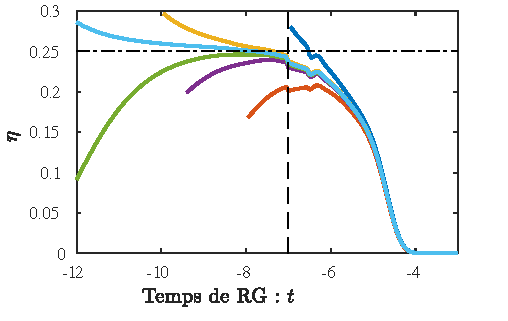
\includegraphics[scale=0.7]{MesuRes.pdf}
\end{center}
\caption{Évolution de $\eta_k$ en fonction de $t$ pour différentes valeurs de la températue $T$.}
\label{fig:etaMesu}
\end{figure}

$\bullet$ Encadrement de la température critique
\begin{equation}
2.350 \, J/k_B < T_c^{BMW}  < 2.375 \, J/k_B
\end{equation}

$\bullet $ Comparaison à la température théorique attendue
\begin{equation}
	err = \frac{ |T_c^{BMW} - T_c^{th}|}{T_c^{th}} \sim 4 \%
\end{equation}



	
	\end{frame}
	
	
	\section{Conclusions}
		\begin{frame}
	\justifying
	\vspace*{22pt}
	
	\end{frame}
	
	

\end{document}